\subsubsection{Dynamik von NCE-Systemen}
Konkrete Erweiterung der Petrinetz-Dynamik bei NCE-Systemen \beiblatt{2-17}

\subsubsection{Beispiel aus NCE-Systemen}
Ampelanlage \beiblatt{2-18}

%TODO Abb

\subsubsection{Transformationen}

\begin{descFixed}[2]
	\item[Problem:] spezielle Kantenarten (Test-/Inhibitor-Kanten, Condition-/Event-Kanten) für die Analyse (s. Kapitel 4) problematisch
	\item[Abhilfe:] Transformation auf PN ohne spezielle Kanten (S/T-Netze) möglich. \beiblatt{2-19}
\end{descFixed}

\includepdf[pages={27 - 29}]{material/AEH_2019.pdf}

\section{Ereignisdiskrete Prozessmodellierung}
\properparagraph{Modellierungsaspekte}
\begin{itemize}
	\item Abbildung des ungesteuerten Prozesses erforderlich ($\Rightarrow$ separater Steuerungsentwurf/Austausch der Steuerung möglich)
	\item explizite Berücksichtigung der gewünschten ($\leftarrow$ Zielstellung) und der verbotenen ($\leftarrow$ Beschränkungen) Prozesssituationen
	\item In der Regel Modularisierung erforderlich: Abgrenzung von Teilsystemen mit Erfassung der zugehörigen Interaktionen
\end{itemize}

Verschiedene Ableitungen von DES-Modellen durch Abstraktion denkbar:

%TODO Abb.

hier: Unterscheidung
\begin{enumerate}
	\item Zustandsorientierte Modellierung
	\item Prozessorientierte Modellierung
\end{enumerate}
jeweils an exemplarischen Prozessen vorgeführt.

\subsection{Zustandsorientierte Modellierung}
\properparagraph{Vorgehensweise:}
\begin{itemize}
	\item Festlegung von Zustandsgrößen \beiblatt{1-5} als prozessrelevante Größen
	\item Bestimmung der diskreten Werte der Zustandsgrößen mit Ereignisdefinition ($\hat{=}$ Zustandsänderungen (extern/autonom))\\
	(falls nicht unmittelbar vorhanden: Abstraktion durch Partitionierung des kontinuierlichen Zustandsraums in Hyperkuben)
	%TODO Abb
\end{itemize}

\properparagraph{Technisches Beispiel:} DES-Modellierung einer Tankbefüllung \beiblatt{3-1}

\subsubsection{Tankbefüllung: Modellierung als Automat}

%TODO Abb

\properparagraph{Kennzeichen}
\begin{itemize}
	\item Mealy-Automat
	\item Ausgabe des Automaten: Sensorik (Sensor a) als Prozessmessgröße (autonomes Ereignis)
	\item Aktorik (=Ventil)-Zustände nicht explizit modelliert, nur durch Änderung der Ereignisse (extern bzw. gesteuert) (sonst Automatengraph zu umfangreich!)
\end{itemize}

\subsubsection{Tankbefüllung: Modellierung als PN bzw. NCE-System}
Ansatz: modularer Aufbau mit Teilnetzen (Ventil berücksichtigt) \beiblatt{3-2 oben}

Modulkopplung auf unterschiedliche Arten möglich:
\begin{enumerate}
	\item \underline{Hinzufügen zusätzlicher (normaler) Kanten} \beiblatt{3-2 unten}
	%TODO Abb.
	
	\properparagraph{Kennzeichen:}
	\begin{itemize}
		\item Verknüpfungen unübersichtlich
		\item Schleifenbildung
		\item Ursache/Folgen-Kopplung
	\end{itemize}
\end{enumerate}

\includepdf[pages={30 - 31}]{material/AEH_2019.pdf}